\begin{figure}[b]
    \centering
    \subfloat[fovea]{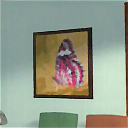
\includegraphics[width=0.3\linewidth]{TOG/figs/layer_blend/lobby_view0000_fovea.png}\label{fig:system:fovea}}\hspace{1em}
    \subfloat[mid-periphery]{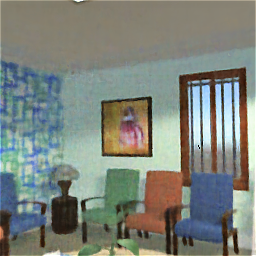
\includegraphics[width=0.3\linewidth]{TOG/figs/layer_blend/lobby_view0000_mid.png}\label{fig:system:mid}}\hspace{1em}
    \subfloat[far-periphery]{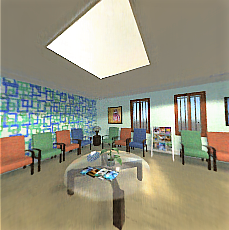
\includegraphics[width=0.3\linewidth]{TOG/figs/layer_blend/lobby_view0000_periph.png}\label{fig:system:far}}
    
    \subfloat[display image]{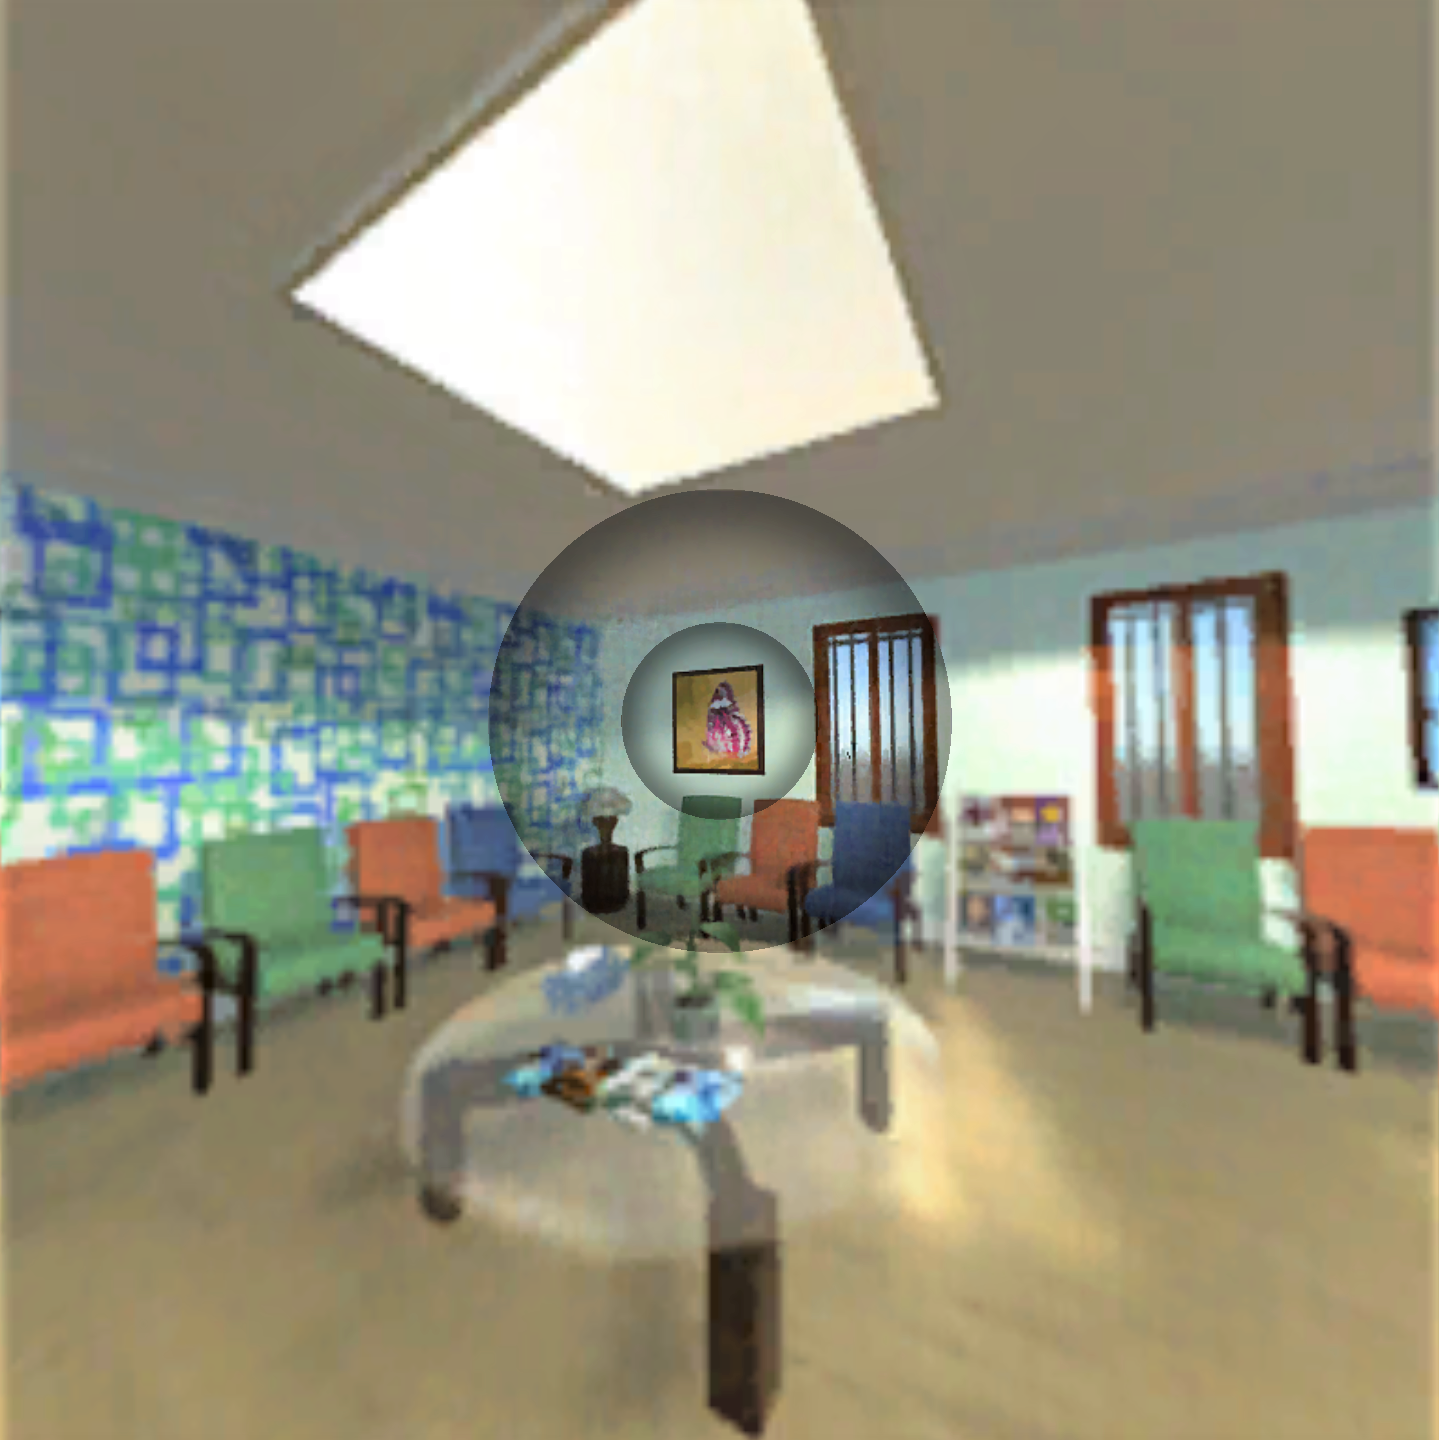
\includegraphics[width=0.9\linewidth]{TOG/figs/layer_blend/lobby_view0000_blendmask.png}\label{fig:system:blending}}
    \Caption{Visual acuity adaptive synthesis and rendering mechanism.}
    {%
    \subref{fig:system:fovea}/\subref{fig:system:mid}/\subref{fig:system:far} shows our individual gaze-contingent synthesis for fovea (within $20$ deg)/mid-periphery (within $45$ deg)/far-periphery (within $110$ deg, the capability of our VR display), respectively. 
    \subref{fig:system:blending} illustrates our real-time rendering system by dynamically blending the individual images to the final displayed frame.
    }
    \label{fig:system}
\end{figure}